% Duck Live, emotions and idle life: the animation layer on top of the RL policies.
% Build:  cd docs && make        Numbers: app/bench_anim.py -> duck_anim_numbers.tex, duck_anim_*_table.tex
\documentclass[11pt]{article}
\usepackage[margin=1in]{geometry}
\usepackage{amsmath,amssymb}
\usepackage{booktabs}
\usepackage{longtable}
\usepackage{graphicx}
\usepackage{xcolor}
\usepackage[colorlinks=true,linkcolor=blue,citecolor=blue,urlcolor=blue]{hyperref}
\usepackage{enumitem}
\usepackage{array}

\newcommand{\code}[1]{\texttt{\small #1}}
\newcommand{\fig}[1]{Fig.~\ref{fig:#1}}
\newcommand{\tab}[1]{Table~\ref{tab:#1}}
% generated by app/bench_anim.py -- do not edit
\newcommand{\animClips}{27}
\newcommand{\animTrials}{920}
\newcommand{\animFalls}{1}
\newcommand{\animDone}{919}
\newcommand{\animStandTrials}{540}
\newcommand{\animStandFalls}{1}
\newcommand{\animSeatedTrials}{380}
\newcommand{\animSeatedFalls}{0}
\newcommand{\animN}{20}
\newcommand{\animNalt}{6}
\newcommand{\animRmseDirect}{0.070}
\newcommand{\animRmseCmd}{0.242}
\newcommand{\animTiltMax}{107.0}
\newcommand{\headRmseStandingCmd}{0.292}
\newcommand{\headRmseStandingDirect}{0.035}
\newcommand{\headRmseSeatedCmd}{0.109}
\newcommand{\headRmseSeatedDirect}{0.035}
\newcommand{\idleSeeds}{8}
\newcommand{\idleMinutes}{10}
\newcommand{\idleFalls}{0}
\newcommand{\idleFallsBare}{0}
\newcommand{\idleDrift}{9.7}
\newcommand{\idleDriftMax}{22.0}
\newcommand{\idleDriftBare}{0.2}
\newcommand{\idleTilt}{4.8}
\newcommand{\idleTiltBare}{2.3}
\newcommand{\idleGlances}{20.0}
\newcommand{\idleYawStd}{0.24}
\newcommand{\idleYawStdBare}{0.008}
\newcommand{\idleYawP}{0.41}
\newcommand{\idleViewer}{8}
\newcommand{\idleBeak}{31}
\newcommand{\dozeAfter}{33}
\newcommand{\dozeN}{8}
\newcommand{\dozeFalls}{0}
\newcommand{\dozePitch}{0.44}
\newcommand{\walkLiveFalls}{0}
\newcommand{\walkLiveVx}{0.018}
\newcommand{\walkLiveWz}{0.371}
\newcommand{\walkLiveTilt}{4.0}
\newcommand{\walkLiveTiltMax}{11.5}
\newcommand{\pushLiveFell}{19}
\newcommand{\pushLiveUp}{32}
\newcommand{\pushLiveT}{0.68}
\newcommand{\walkBareFalls}{0}
\newcommand{\walkBareVx}{0.026}
\newcommand{\walkBareWz}{0.215}
\newcommand{\walkBareTilt}{3.8}
\newcommand{\walkBareTiltMax}{9.3}
\newcommand{\pushBareFell}{14}
\newcommand{\pushBareUp}{32}
\newcommand{\pushBareT}{0.76}
\newcommand{\walkN}{16}
\newcommand{\pushN}{32}
\newcommand{\reactN}{20}
\newcommand{\reactJumpLanded}{20}
\newcommand{\reactJump}{20}
\newcommand{\reactJumpT}{0.02}
\newcommand{\reactFlipLanded}{20}
\newcommand{\reactFlip}{20}
\newcommand{\reactFlipT}{0.02}
\newcommand{\reactFell}{18}
\newcommand{\reactUp}{18}
\newcommand{\reactShook}{18}
\newcommand{\deadN}{20}
\newcommand{\deadUp}{20}
\newcommand{\deadT}{1.19}
\newcommand{\deadTmax}{1.22}
\newcommand{\faceYawA}{2.20}
\newcommand{\faceYawB}{0.27}
\newcommand{\faceYawBmax}{0.29}
\newcommand{\faceT}{2.23}
\newcommand{\faceOk}{20}
\newcommand{\faceFalls}{0}
\newcommand{\cutClip}{0.86}
\newcommand{\cutNone}{0.71}
\newcommand{\cutOk}{20}
\newcommand{\bodyDzMax}{0.3}
\newcommand{\bodyPitchMax}{3.1}
\newcommand{\bodyWalkMax}{320}
\newcommand{\bodyReps}{6}
\newcommand{\costBare}{0.58}
\newcommand{\costLive}{0.62}
\newcommand{\costClip}{0.63}

\makeatletter\newcommand{\rowsfrom}[1]{\@@input #1.tex }\makeatother   % \input inside a tabular breaks \bottomrule

\title{Duck Live, emotions and idle life:\\ an animation layer that leaves the legs to the RL policies}
\author{microduck\_replication\_feetech}
\date{\today}

\begin{document}
\sloppy
\maketitle

\begin{abstract}
The Duck Live app (\code{docs/duck\_live\_app.pdf}) drives the HD1910 Microduck replica's reinforcement-learning
policies from the keyboard. This document adds a character on top of them: \animClips~emotion clips---Pollen
Robotics' 14 open-source Microduck emotions and 13 written here---an idle life that keeps the duck looking around,
breathing, glancing at the viewer and dozing off, and reactions to what just happened to it. The layer never takes
the legs: at every 50~Hz tick it only chooses four neck/head joint offsets, a beak opening, optionally a twist for
the walk policy, and when to fire the sit, jump and front-flip policies; the active policy sees the moving head in
its joint observations and balances against it. Measured on the app's MuJoCo plant: the VelStand walk does not track
its own head command on this checkpoint (\headRmseStandingCmd~rad RMS error against \headRmseStandingDirect~rad
when the head servos are driven directly), so standing the head is driven directly; over \animTrials~jittered trials
of every clip the duck fell \animFalls~times and \animDone~clips ran to their end, with a mean head tracking error
of \animRmseDirect~rad; \idleSeeds$\times$\idleMinutes~minutes of idle life produced \idleFalls~falls and
\idleDrift~cm of drift; walking with the idle life on changes the forward-speed error from \walkBareVx{} to
\walkLiveVx~m/s; and the one clip that switches the policies off, playing dead, ended with the stand-up policy
getting the duck back on its feet \deadUp/\deadN~times in \deadT~s. The control tick costs \costLive~ms with the
layer on against \costBare~ms without. The beak is drawn, not simulated: the MJCF has no jaw joint.
\end{abstract}

\par\smallskip\noindent\textbf{Keywords:} expressive robot motion, character animation, bipedal robot, reinforcement
learning policy, head motion as disturbance, idle behaviour, Microduck, MuJoCo.\par\smallskip

\section{Overview}
A robot that stands perfectly still reads as switched off; one that sweeps its head on a sinusoid reads as a machine.
Expressive motion for legged characters is usually obtained by training the policy on the animation itself
\cite{bdx}; here the policies already exist and are not retrained. The Microduck's training recipe leaves a way in:
the observation carries a 4-wide head command and a 6-wide body-pose command next to the twist
(\code{docs/duck\_live\_app.pdf}, \S2.2), and Pollen's runtime plays its emotions by writing those commands
\cite{emotions,microduck}. What this checkout's policies actually do with those commands had not been measured;
\S\ref{sec:exp} does, and the design follows from it.

The pieces (all in \code{app/}):
\begin{itemize}[nosep]
\item \code{animations/} --- the clip library: keyframes (Pollen's format), sounds, \code{manifest.json}. Built by
  \code{tools/make\_animations.py}: Pollen's 14 emotions copied unchanged (Apache-2.0, licence included), the 13
  originals generated from control points, with voices synthesised by Pollen's own voice synth
  (\code{tools/quack.py}, the robot's personality seed) and the beak lip-synced to the sound.
\item \code{animation.py} --- the runtime: \code{Clip}, \code{IdleLife}, \code{Animator}.
\item \code{engine.py} --- applies the layer's output inside \code{Duck.step} (\S\ref{sec:apply}); hosts the
  scripted pose of the play-dead clip.
\item \code{web/index.html} --- the emotion palette, the beak, the voice (Web Audio), particles and the bubble.
\item \code{bench\_anim.py} --- every number and figure below.
\end{itemize}

\section{Method}\label{sec:method}
\subsection{What the layer controls}
Let $q_h\in\mathbb{R}^4$ be the neck-pitch, head-pitch, head-yaw and head-roll joint angles and $\bar q_h$ their
default pose. The layer outputs, every control tick ($\Delta t = 20$~ms),
\[
  h\in\mathbb{R}^4 \ \text{(desired offset } q_h-\bar q_h\text{)},\qquad m\in[0,1]\ \text{(beak)},\qquad
  \tau\in\mathbb{R}^3\cup\{\varnothing\}\ \text{(twist } v_x,v_y,\omega_z\text{)},
\]
and discrete skill requests (sit, jump, flip). Sign conventions are Pollen's: head pitch $>0$ is beak down, head yaw
$>0$ is to the duck's left. Everything else---the ten leg joints always, and the head whenever the layer's weight is
zero---is the active policy's action.

\subsection{Clips}
A clip is a sequence of keyframes $(t_k, h_k, m_k, \tau_k, s_k)$, sampled every 0.1~s (Pollen's files) or 0.05~s
(the originals) and interpolated linearly, plus one or more sound files started at $t=t_\text{sound}$ (several
voicings: one is drawn at random). $s_k$ is an optional skill. Pollen's keyframes also carry a body pitch $b_k$ and
height; the body-pose command they are meant for is not usable on this checkpoint (\S\ref{sec:exp:body}), so the bow is
shown with the head instead, $h^\text{pitch}_k \leftarrow h^\text{pitch}_k + 0.6\,b_k$, and the height is dropped.

The originals are written as control points per channel joined by minimum-jerk segments \cite{minjerk},
$x(u) = x_0 + (x_1-x_0)(10u^3-15u^4+6u^5)$, plus windowed oscillations
$a\,e^{-\lambda (t-t_0)}\sin(2\pi f (t-t_0)+\varphi)$ for shakes, wiggles and sways. Their beak track is the
maximum of what the clip opens by hand and a lip-sync term $0.85\,(e(t+30~\text{ms})/\max e)^{0.6}$, where $e$ is
the 30~ms RMS envelope of the clip's own sound (the 30~ms lead covers the beak's slew).

Timeline rules, the same as Pollen's player where they overlap: a clip starts only from a quiet stand (or seated,
for clips that need neither legs nor a skill); a walking duck is not interrupted by an automatic reaction, and a
manual request waits up to 6~s for the duck to stop or stand up; a jump or flip fired by a clip pauses the clip's
clock until the walk policy has the duck back (at most 6~s); a fall, or the user's own S / space / R, ends the
clip; an arrow key ends it at once (the user is driving). A clip marked \emph{face} first turns the body towards
the viewer with the walk policy ($\omega_z=\operatorname{sign}(\psi)\min(1, 0.45+0.6|\psi|)$~rad/s while the
viewer's bearing $|\psi|>0.7$~rad, until $|\psi|<0.3$~rad or 4.5~s), then adds the remaining bearing to its head
yaw.

\subsection{Idle life}\label{sec:idle}
\code{IdleLife} follows the ideas of Pollen's \code{idle\_head.rs} \cite{microduck} (re-implemented; it adds the
viewer, the turn lead and the grab). Five channels (neck, pitch, yaw, roll, beak):
\begin{itemize}[nosep]
\item \textbf{Glance.} When the current hold expires a new target is drawn: with probability 0.30 the viewer (if
  its bearing is within 2.0~rad; the head turns at most 1.05~rad for it), 0.16 the middle, otherwise a yaw of
  0.18--0.62~rad times the reach $\rho$, preferring the other side, and a pitch in $[-0.22, 0.14]\rho$; a roll of
  0.10--0.24~rad on 28\% of glances; a small neck lean and beak opening. Travel is minimum-jerk over
  $0.22$--$0.42~\text{s}+0.30|\Delta\text{yaw}|$; the hold is 0.7--2.8~s divided by $(0.45+0.55E)$.
\item \textbf{Re-fixation.} Every 0.35--0.95~s during a hold the gaze shifts by up to 0.035~rad (yaw) and 0.02~rad
  (pitch), first-order filtered (60~ms).
\item \textbf{Drift and breath.} Four incommensurate sines of 0.01--0.02~rad, and a breath of period 3.4~s that moves
  the neck by 0.016~rad and counter-rotates the head pitch so the face stays level.
\item \textbf{Energy.} $E = (0.35+0.65\,e^{-t_\text{still}/45~\text{s}})(1+0.35M)$ scales the reach; $M\in[-1,1]$ is
  a mood left by the last clip (sad: head 0.1~rad lower, slower; happy: chin up, livelier) that decays with a 25~s
  time constant.
\item \textbf{Dozing.} Seated and still for 25~s the head sinks 0.5~rad, the glances all but stop and the breath
  slows; any key wakes it.
\item \textbf{Walking.} The reach drops to 45\%, and the head leads the turn: yaw $+0.38\,\hat\omega_z$, roll
  $+0.07\,\hat\omega_z$, with $\hat\omega_z$ the commanded yaw rate low-passed at 0.18~s. Under run, sprint, jump,
  flip and stand-up the policy keeps its own head.
\item \textbf{Grab.} While the user pulls the duck with the spring the head turns to the pull point and the beak
  opens.
\end{itemize}
The generator is seeded; for a given seed and input sequence the layer is deterministic.

\subsection{Reactions}
With reactions on, an event queues a clip: back on its feet after a fall $\to$ \emph{shake off}; a jump that took off
and landed $\to$ \emph{yep}; a jump that did not take off $\to$ \emph{mmh?}; a landed flip $\to$ \emph{proud}; let go
after a pull longer than 1~s $\to$ \emph{mmh?}; 40--70~s of standing with nothing to do $\to$ a yawn. Tricks fired
by a clip itself raise no reaction, and a reaction never starts while a key is held.

\subsection{How the offsets reach the servos}\label{sec:apply}
The clip and idle outputs are cross-faded (weight $c$, 0.18~s), limited, and slewed:
\[
  h^\star = c\,h_\text{clip} + (1-c)\,h_\text{idle},\qquad
  h \leftarrow h + \operatorname{clip}\!\big(\operatorname{clip}(h^\star, h_\text{lo}, h_\text{hi}) - h,\ \pm 12~\text{rad/s}\cdot\Delta t\big).
\]
The limits are $[-0.45, 0.30]$, $[-0.75, 1.00]$, $\pm1.20$, $\pm0.42$~rad standing and $[-0.80, 0.45]$,
$[-0.75,1.00]$, $\pm1.50$, $\pm0.42$ seated. The standing neck limit is the measured one: further forward the head's
mass moves the centre of mass enough that VelStand steps to stay up, which Pollen also reports on the real duck
\cite{emotions}. An override weight $w\in[0,1]$ fades in (0.2~s) while a clip plays or the idle life is on, in the
states stand, stopping, walk, seated and (for a clip) sitting down, and fades out when the duck is down, when the
trunk tilts past $30^\circ$ (the policy may need its head to catch itself), and under every policy that is not walk
or sit-stand. With $a$ the policy's action and $\bar q$ the default pose, the servo target $q^\star$ and the
observation's head command $c_h$ are
\[
\text{walk (VelStand):}\quad q^\star_h = (1-w)(\bar q_h + a_h) + w(\bar q_h + h),\quad c_h = 0;\qquad
\text{sit-stand:}\quad q^\star = \bar q + a,\quad c_h = w\,h .
\]
The choice per policy is \S\ref{sec:exp:head}. In both cases the leg targets are $\bar q + a$ untouched, and the
policy observes the true head angles. A clip twist replaces the key-derived twist of the walk policy only while
the operator state is stand or stopping, clipped to the policy's trained ranges; it is not slewed (the clips are
already smooth).

\subsection{Playing dead}
One clip leaves the policies: Pollen's \emph{play dead} gives two timed joint poses (legs straight, then legs up)
with the head limp. From the first stage the engine holds a scripted target---the listed joints ramp linearly from
their current angle over the stage's ramp time, the limp joints' targets follow their encoders, the rest hold---and
runs no policy; fall detection is off. Any key hands the duck to the stand-up policy as if it had fallen. The stages
use the simulation timings of the source (1.8~s and 4.0~s are the robot's).

\subsection{Beak}
Pollen's MJCF welds the jaw into the head body, so there is no joint to drive. The page hangs the two lower-beak
meshes (\code{jaw}, \code{jaw\_soft}) from a pivot at the beak servo's axis (head frame: $x=3.2$~mm, $z=-18$~mm,
axis $+y$) and rotates them by $0.42\,m$~rad; $m$ is slewed at 14~s$^{-1}$. The jaw's mass stays where the policies
trained with it. This is a rendering, with no contact and no dynamics.

\section{Experiments}\label{sec:exp}
All runs: \code{app/bench\_anim.py}, the app's plant (C~MuJoCo~\cite{mujoco}, BAM HD1910 servos, 0.005~s physics, 50~Hz control),
policies of \code{exports/} at their defaults. A trial starts from a jittered stand ($\pm1^\circ$ on every servo,
$\pm2^\circ$ yaw, a command delay drawn from 3--6 physics steps) and settles for 1~s; seeds are fixed.

\subsection{A. Head offsets: through the policy or straight to the servos}\label{sec:exp:head}
A constant offset on one head joint is held for 3~s, sent either as the policy's head command or as the head servo
targets; the achieved offset is the mean over the last 1.5~s (\fig{head}, \tab{head}). Standing under VelStand the
head command is not tracked: the response is a nonlinear function of the command with dead bands (a $-0.5$~rad yaw
command leaves the head where it was), \headRmseStandingCmd~rad RMS. This checkpoint (iteration 21\,495) was
trained with head commands of at most $\pm0.17$--$0.21$~rad, a stage of a curriculum that widens later. Driving the
servos directly gives \headRmseStandingDirect~rad with the policy holding the stand. Seated, the sit-stand policy
tracks its command (\headRmseSeatedCmd~rad) and saturates what it cannot balance: a neck command of $-0.8$~rad
yields about $-0.5$. Driving the servos directly seated is more accurate within $\pm0.45$~rad but it is the larger
neck offsets that matter there, and those are the ones the policy declines. Hence \code{HEAD\_MODE}: direct for
walk, command for sit-stand.
\begin{figure}[h]\centering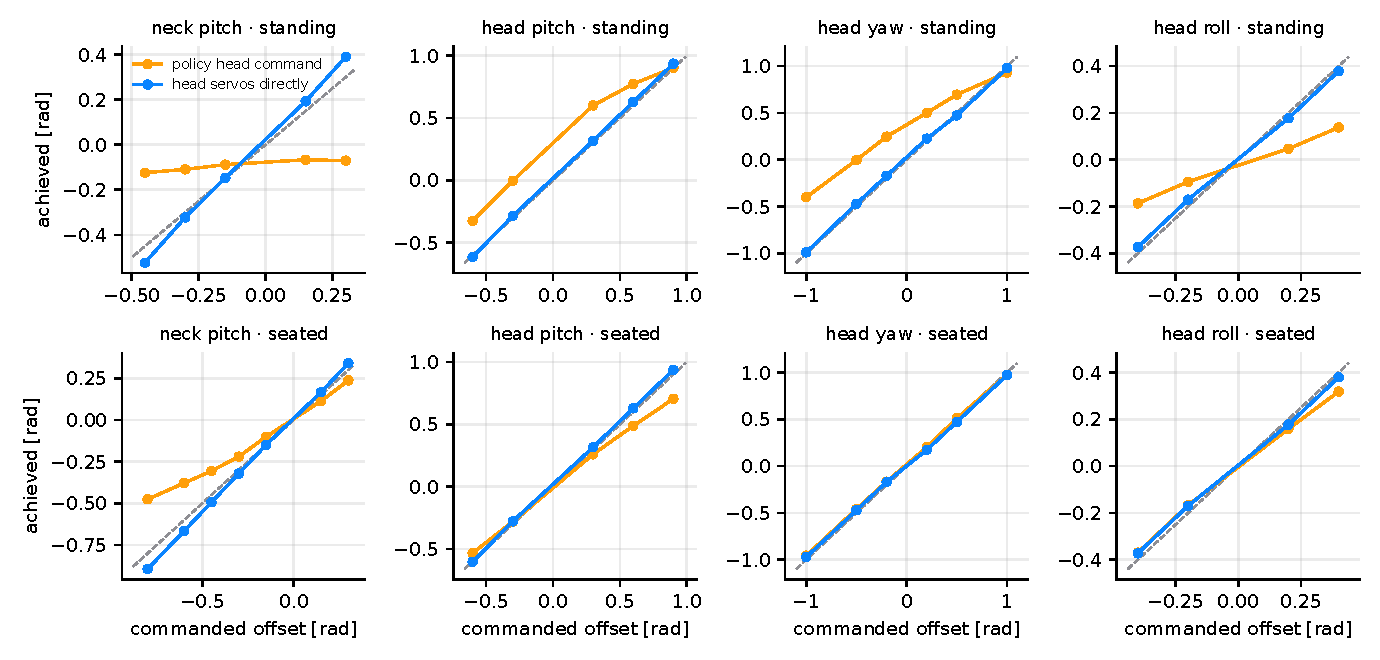
\includegraphics[width=0.95\linewidth]{figures/duck_anim_head_tracking.pdf}
\caption{Achieved against commanded head offset, per joint. Top: standing (VelStand). Bottom: seated (sit-stand). A
red cross marks a fall.}\label{fig:head}\end{figure}
\begin{table}[h]\centering\small
\begin{tabular}{lrrrr}\toprule
posture, path & RMSE [rad] & worst tilt [deg] & mean drift [m] & fell\\\midrule
\rowsfrom{duck_anim_head_table}\bottomrule\end{tabular}
\caption{Head offset tracking over all joints and amplitudes.}\label{tab:head}\end{table}

\subsection{B. The body-pose command}\label{sec:exp:body}
Each of the six body-pose slots is held at either end of its training range for 3~s, \bodyReps~starts each
(\tab{body}). No slot moves the trunk height by more than \bodyDzMax~mm, the pitch response is at most
\bodyPitchMax$^\circ$ and asymmetric, and one setting (slot 3 at $-0.05$) makes the duck turn and walk
\bodyWalkMax~mm away from a zero twist. The command is therefore left at zero and the clips' body pitch is folded into the head.
\begin{table}[h]\centering\small
\begin{tabular}{rrrrrrr}\toprule
slot & value & $\Delta z$ [mm] & nose-down [deg] & roll [deg] & yaw [deg] & walked [mm]\\\midrule
\rowsfrom{duck_anim_bodypose_table}\bottomrule\end{tabular}
\caption{VelStand's response to its body-pose command (slots 0--2 in metres, 3--5 in radians), relative to the
zero-command stand.}\label{tab:body}\end{table}

\subsection{C. Every clip}\label{sec:exp:clips}
Each clip is played \animN~times from a jittered stand, and seated for the clips that allow it, with the idle life
on; the trial runs until 2.5~s after the clip (\tab{clips}, \fig{clips}). Over \animTrials~trials the duck fell
\animFalls~times (\animStandFalls/\animStandTrials~standing, \animSeatedFalls/\animSeatedTrials~seated) and
\animDone~clips ran to their last keyframe. The one fall is \emph{happy}: in one of its 20 trials the jump it
fires ended on the floor (the jump policy itself lands 94\% of its jumps in training), the stand-up policy took over
and the clip was abandoned; that trial is the \animTiltMax$^\circ$ worst tilt of the table. Head
tracking error is the RMS difference between the measured head joints and the layer's (limited, slewed) output
while the clip has the head: \animRmseDirect~rad averaged over the head-only clips, against \animRmseCmd~rad for the
same clips sent through VelStand's head command (\animNalt~trials each). Standing, the remaining error is the
servo: the largest values are on the fast yaw shakes (\emph{angry}, \emph{excited}), which ask for up to 7~rad/s.
Seated, the largest are the deep neck droops (\emph{sad}, \emph{curious}, \emph{devastated}), which the sit-stand
policy declines to follow all the way (\S\ref{sec:exp:head}). \fig{trace}
shows one clip. The clips that use the policies behave as written: \emph{happy} wiggles on the walk policy and
jumps, \emph{show off} flips, \emph{nap}, \emph{devastated} and \emph{play dead} sit; the drift column is the
distance the clip moves the duck (the hop back of \emph{startled}, the landing of the flip).
\begin{figure}[h]\centering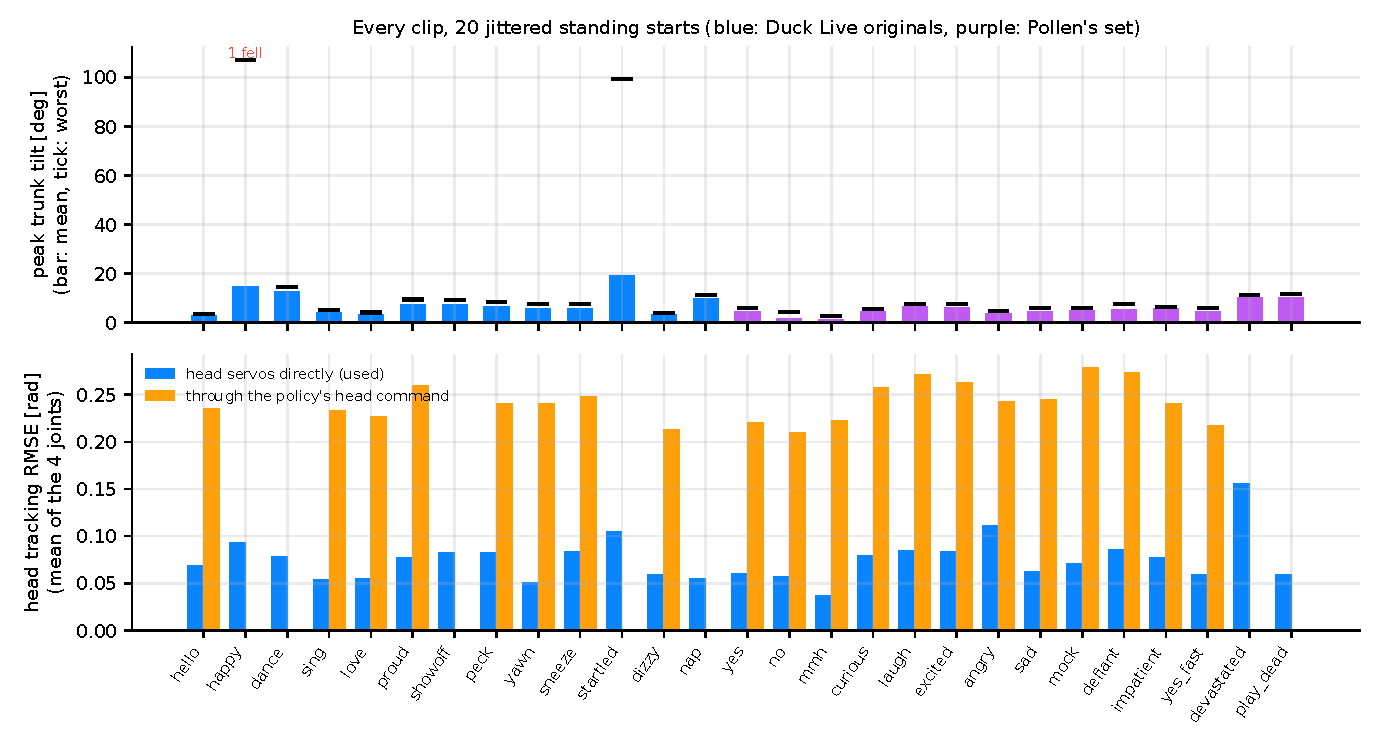
\includegraphics[width=0.95\linewidth]{figures/duck_anim_clips.pdf}
\caption{Per clip, standing starts: peak trunk tilt, and head tracking error under the two head paths (clips with a
skill, a twist or a scripted pose are not run through the command path).}\label{fig:clips}\end{figure}
\begin{figure}[h]\centering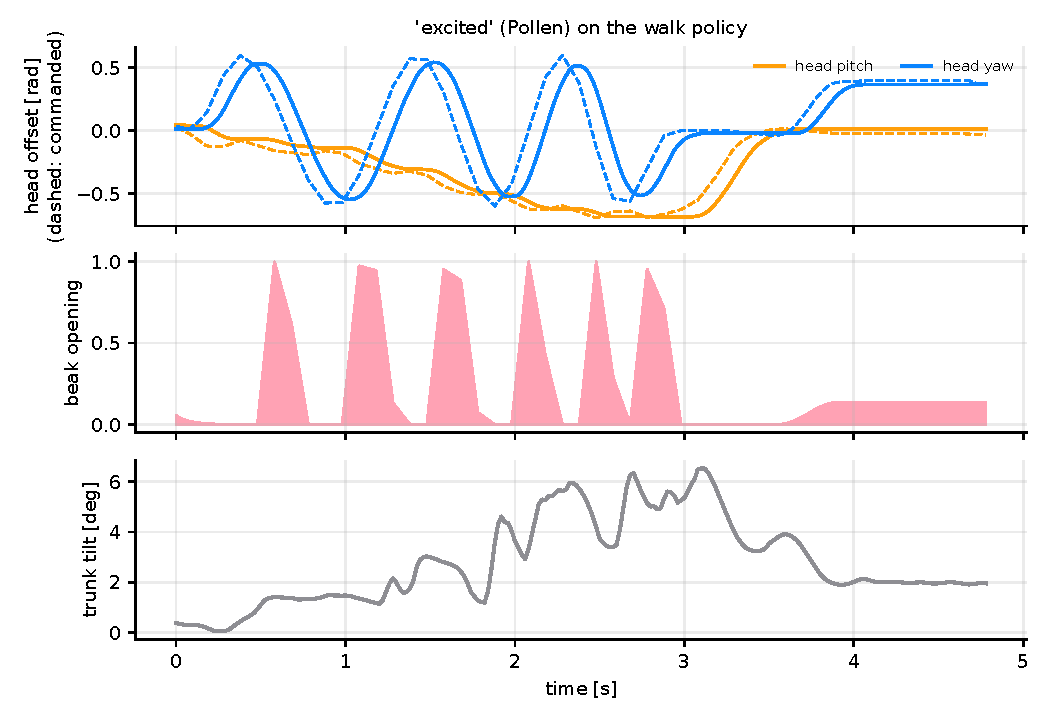
\includegraphics[width=0.7\linewidth]{figures/duck_anim_clip_trace.pdf}
\caption{One clip in detail: commanded and measured head offsets, beak opening, trunk tilt.}\label{fig:trace}\end{figure}

{\footnotesize\setlength{\tabcolsep}{4pt}
\begin{longtable}{llrrrrrrrl}
\caption{Every clip. DL: Duck Live original, P: Pollen. Tilt: mean / worst peak over the trials. RMSE: mean of the
four head joints.}\label{tab:clips}\\\toprule
clip & src & start & $T$ [s] & falls & done & tilt [deg] & drift [m] & RMSE [rad] & skills fired\\\midrule\endhead
\rowsfrom{duck_anim_clip_table}\bottomrule
\end{longtable}}

\subsection{D. Idle life}
\idleSeeds~seeds of \idleMinutes~minutes standing with the idle life on, the viewer placed on a 0.9~m circle at a
different bearing per seed, against the bare policy (\fig{idle}): \idleFalls~falls (bare: \idleFallsBare), drift
\idleDrift~cm on average and \idleDriftMax~cm at most (bare: \idleDriftBare~cm), worst tilt \idleTilt$^\circ$
(bare: \idleTiltBare$^\circ$). The head makes \idleGlances~glances per minute, its yaw has a standard deviation of
\idleYawStd~rad (bare: \idleYawStdBare) with 95\% of the time inside $\pm$\idleYawP~rad, it is on the viewer
\idleViewer\% of the time and the beak is open \idleBeak\% of the time. The drift is the cost: a head turned far to
one side shifts the support and VelStand shuffles; it is largest for the seeds whose viewer stands behind the duck,
where every look at the viewer is a look over the shoulder. Seated for 3~minutes, \dozeN/\idleSeeds~seeds
dozed off after \dozeAfter~s with the head \dozePitch~rad down and \dozeFalls~falls.
\begin{figure}[h]\centering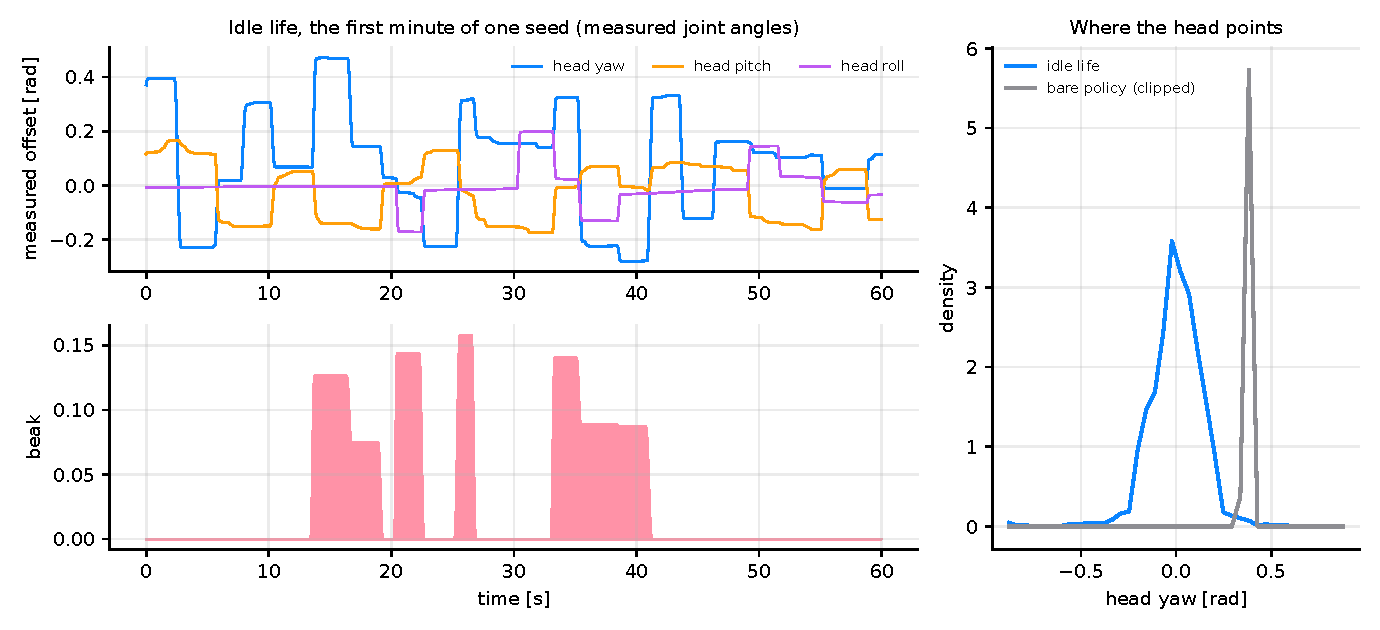
\includegraphics[width=0.95\linewidth]{figures/duck_anim_idle.pdf}
\caption{Idle life. Left: measured head joints and beak over the first minute of one seed. Right: distribution of
the head yaw over all seeds.}\label{fig:idle}\end{figure}

\subsection{E. Driving and pushes with the idle life on}
A driving scenario (forward 2.5~s, forward-left 2.5~s, forward-right 2~s, turn left 2~s, back 1.5~s, release) over
\walkN~identical jittered starts with and without the idle life: falls \walkLiveFalls{} against \walkBareFalls;
forward-speed RMS error \walkLiveVx{} against \walkBareVx~m/s; yaw-rate RMS error \walkLiveWz{} against
\walkBareWz~rad/s; mean trunk tilt \walkLiveTilt$^\circ$ against \walkBareTilt$^\circ$. Pushes of 1.0--2.5~m/s on the
standing duck, \pushN~per condition (the same pushes): \pushLiveFell~fell with the idle life on and
\pushBareFell~without; \pushLiveUp{} and \pushBareUp~were standing 2~s later; the get-up took \pushLiveT{} and
\pushBareT~s. So the idle life is not free while driving: forward speed is unaffected, but the yaw rate oscillates
more around its command with the head leading the turn, and a head that is off-centre when the push arrives makes a
fall more likely. No scenario run fell, and every pushed duck was back up. The head override is released above
$30^\circ$ of tilt, so a falling duck has its policy's head.

\subsection{F. Reactions, the turn to the viewer, play dead, interruption}
\reactN~trials each. Space: \reactJumpLanded~landed, \reactJump~reactions, \reactJumpT~s after the hand-back. R:
\reactFlipLanded~landed, \reactFlip~reactions. A 3~m/s push: \reactFell~fell, \reactUp~got up, \reactShook~shook
it off. \emph{Hello} with the viewer \faceYawA~rad round (the app's default camera, behind the duck): the walk policy
turned the duck to \faceYawB~rad (\faceYawBmax~at worst) in \faceT~s and the greeting started \faceOk~times, with
\faceFalls~falls. \emph{Play dead}: \deadN~ended on their backs with the policies off; after the wake key the
stand-up policy had \deadUp~standing in \deadT~s (\deadTmax~at most). An arrow key pressed 2~s into \emph{sad}: the
clip ended on that tick in \cutOk~trials and the duck reached 80\% of the 0.4~m/s command after \cutClip~s, against
\cutNone~s from the idle stand.

\subsection{G. Cost}
Median control tick: \costBare~ms with the bare policy, \costLive~ms with the idle life, \costClip~ms with a clip
playing.

\section{Implementation and usage}
\begin{verbatim}
app/ducklive.sh               # the app; emotions on the left panel
app/tools/make_animations.py  # rebuild app/animations/
app/bench_anim.py [--quick] [--only headtrack,clips,idle,walk,
                              reactions,cost,bodypose]
\end{verbatim}
Keys: the number row plays Pollen's short expressions (1 yes, 2 no, 3 mmh, 4 curious, 5 laugh, 6 excited, 7 angry,
8 sad, 9 mock, 0 defiant), K impatient, L yep, Z devastated, X play dead; Q hello, W happy, E dance, T sing, Y love,
U proud, I show off, O peck, P yawn, F sneeze, G startled, H shake off, J nap; M mutes. The chips \emph{alive}
and \emph{reacts} switch the idle life and the reactions (\code{server.py --still --no-react} starts without
them). The engine API is \code{Duck(lively=, react=, anim\_seed=)}, \code{duck.emote(name)},
\code{duck.anim.viewer\_pos}; with both switches off and no clip requested the engine is exactly the policies,
which is how \code{bench\_mac.py} runs. The WebSocket gains \code{\{"t":"emote","name":\ldots\}} and
\code{\{"t":"cam","pos":\ldots\}}; each snapshot carries the beak opening, the playing clip and the id of the
last sound started, which the page plays with Web Audio.

A new clip is two files and a manifest entry in Pollen's format; the fields this player adds are a per-keyframe
\code{twist} and the skills \code{jump} and \code{flip}. On the real robot the same clips go through Pollen's
\code{robotd} emotion player \cite{microduck}; the head path would need the measurement of \S\ref{sec:exp:head}
repeated on hardware, because there the head offsets are sent as the policy's head command.

\section{Limitations}
\begin{itemize}[nosep]
\item \textbf{The beak is not simulated.} No jaw joint, mass shift, contact or grasp; the opening is a rendering.
\item \textbf{Driving the head servos directly is outside the policy's training distribution} in the sense that the
  policy's own head action is discarded. It balances against the result in every trial here, on this plant; the
  standing neck limit and the $30^\circ$ release are what keep it there. This is not validated on the real robot.
\item \textbf{Pollen's clips are not played as authored} where they exceed this plant's limits (the neck reach of
  \emph{curious}, \emph{sad}, \emph{devastated}) and their body pitch and height are shown as head pitch or dropped.
\item \textbf{Idle life costs position and some robustness}: \idleDrift~cm of drift over ten minutes on average
  (\idleDriftMax~cm at worst) against millimetres for the bare policy, a larger yaw-rate error while turning, and
  more falls under pushes (\pushLiveFell{} against \pushBareFell{} of \pushN). The \emph{alive} chip switches it off.
\item \textbf{Clips that fire a trick inherit its failure rate}: \emph{happy} fell once in 20 on its jump.
\item \textbf{Tracking error is dominated by the servo} on the fastest shakes; the clips ask for more head speed
  than the HD1910 model delivers.
\item \textbf{No perception.} The duck looks at the camera position the page reports and at the pull point, nothing
  else; the reactions are a fixed event-to-clip table.
\item \textbf{Sound is the page's}, started from a snapshot field, so it lags the motion by the snapshot and audio
  path latency (not measured).
\end{itemize}

\begin{thebibliography}{9}
\bibitem{emotions} Pollen Robotics. microduck\_emotions: 14 emotions, each a motion and a sound designed together
  (Apache-2.0), 2026. \url{https://github.com/pollen-robotics/microduck_emotions}
\bibitem{microduck} Pollen Robotics. Microduck: a tiny biped duck robot (\code{robotd/src/emotion.rs},
  \code{robotd/src/idle\_head.rs}, the voice synth \code{sounds/}), 2026.
  \url{https://github.com/pollen-robotics/microduck}
\bibitem{bdx} R.~Grandia, E.~Knoop, M.~Hopkins, G.~Wiedebach, J.~Bishop, S.~Pickles, D.~M\"uller, M.~B\"acher.
  Design and control of a bipedal robotic character. Robotics: Science and Systems, 2024.
\bibitem{mujoco} E.~Todorov, T.~Erez, Y.~Tassa. MuJoCo: A physics engine for model-based control. IROS, 2012.
\bibitem{minjerk} T.~Flash, N.~Hogan. The coordination of arm movements: an experimentally confirmed mathematical
  model. Journal of Neuroscience, 5(7), 1985.
\end{thebibliography}
\end{document}
